\section{Image Management}

ส่วนนี้อธิบายการออกแบบและพัฒนา API สำหรับจัดการรูปภาพ ซึ่งเป็นหัวใจหลักของระบบวิเคราะห์เซลล์ โดยครอบคลุมการอัปโหลด จัดเก็บ ดึงข้อมูล และลบรูปภาพ พร้อมทั้งการจัดการ Metadata และความปลอดภัย

% ============================================================================
\subsection{API Endpoints Overview}

\begin{table}[h]
\centering
\caption{Image Management Endpoints}
\begin{tabular}{|l|l|p{6cm}|}
\hline
\textbf{Method} & \textbf{Endpoint} & \textbf{Description} \\
\hline
GET & \texttt{/folders/\{id\}/images} & แสดงรายการรูปภาพในโฟลเดอร์ (Pagination) \\
\hline
POST & \texttt{/folders/\{id\}/images} & อัปโหลดรูปภาพใหม่ (Multipart) \\
\hline
GET & \texttt{/images/\{id\}} & ดูรายละเอียดรูปภาพ \\
\hline
DELETE & \texttt{/images/\{id\}} & ลบรูปภาพ (Cascade) \\
\hline
\end{tabular}
\end{table}

% ============================================================================
\subsection{State Diagram: Image Lifecycle}

รูปภาพในระบบมี State หลายสถานะตลอด Lifecycle:

\begin{figure}[h]
\centering
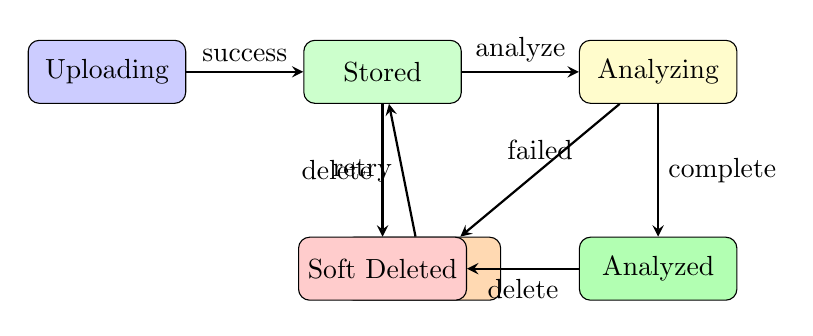
\begin{tikzpicture}[node distance=2.5cm]
    \tikzstyle{state} = [rectangle, rounded corners, draw, minimum width=2cm, minimum height=0.8cm, align=center]
    \tikzstyle{arrow} = [thick,->,>=stealth]
    
    \node (upload) [state, fill=blue!20] {Uploading};
    \node (stored) [state, fill=green!20, right of=upload, xshift=1cm] {Stored};
    \node (analyzing) [state, fill=yellow!20, right of=stored, xshift=1cm] {Analyzing};
    \node (analyzed) [state, fill=green!30, below of=analyzing] {Analyzed};
    \node (error) [state, fill=orange!30, below of=analyzing, xshift=-3cm] {Error};
    \node (deleted) [state, fill=red!20, below of=stored] {Soft Deleted};
    
    \draw [arrow] (upload) -- node[above] {success} (stored);
    \draw [arrow] (stored) -- node[above] {analyze} (analyzing);
    \draw [arrow] (analyzing) -- node[right] {complete} (analyzed);
    \draw [arrow] (analyzing) -- node[above] {failed} (error);
    \draw [arrow] (error) -- node[left] {retry} (stored);
    \draw [arrow] (stored) -- node[left] {delete} (deleted);
    \draw [arrow] (analyzed) -- node[below] {delete} (deleted);
\end{tikzpicture}
\caption{Image Lifecycle State Diagram (with Fault Tolerance)}
\end{figure}

\textbf{หมายเหตุ:} State ``Error'' รองรับกรณี AI Analysis ล้มเหลว (เช่น ไฟล์เสีย, Model timeout) โดยสามารถ retry ได้

% Mermaid version (commented for reference)
% stateDiagram-v2
%     [*] --> Uploading
%     Uploading --> Stored : validation passed
%     Uploading --> [*] : validation failed
%     Stored --> Analyzing : POST /analyze
%     Analyzing --> Analyzed : job completed
%     Analyzing --> Error : job failed
%     Error --> Stored : retry
%     Stored --> SoftDeleted : DELETE request
%     Analyzed --> SoftDeleted : DELETE request
%     SoftDeleted --> [*] : garbage collected

% ============================================================================
\subsection{Sequence Diagram: Image Upload Flow}

% Mermaid Sequence Diagram (commented)
% sequenceDiagram
%     autonumber
%     actor Client
%     participant API as Backend API
%     participant Validator
%     participant Storage as Storage Service
%     participant DB as PostgreSQL
%     
%     Client->>API: POST /folders/{id}/images (multipart)
%     activate API
%     
%     API->>Validator: Validate file type & size
%     alt Invalid file
%         Validator-->>API: Error (invalid type/size)
%         API-->>Client: 400 Bad Request
%     else Valid file
%         Validator-->>API: OK
%     end
%     
%     API->>Storage: Save file to disk/S3
%     activate Storage
%     Storage-->>API: file_path, file_size
%     deactivate Storage
%     
%     API->>API: Extract metadata (width, height)
%     
%     API->>DB: INSERT INTO images
%     activate DB
%     DB-->>API: image record
%     deactivate DB
%     
%     API-->>Client: 201 Created (ImageResponse)
%     deactivate API

\begin{figure}[h]
\centering
\includegraphics[width=0.8\textwidth]{assets/image_upload_sequence.pdf}
\caption{Image Upload Sequence Diagram}
\label{fig:image_upload_seq}
\end{figure}

% ============================================================================
\subsection{Algorithm Analysis}

\subsubsection{File Upload Algorithm}

\begin{lstlisting}[language=Rust, caption=Image Upload Implementation Logic]
async fn upload_image(folder_id, user_id, file) -> Result<Image> {
    // Step 1: Validate ownership - O(log N)
    let folder = verify_folder_ownership(folder_id, user_id)?;
    
    // Step 2: Validate file - O(1)
    validate_file_type(file.mime_type)?;  // Allow: jpeg, png, tiff
    validate_file_size(file.size)?;       // Max: 50MB
    
    // Step 3: Generate unique filename - O(1)
    let uuid = Uuid::new_v4();
    let extension = get_extension(file.mime_type);
    let file_path = format!("{}/{}.{}", STORAGE_PATH, uuid, extension);
    
    // Step 4: Save to storage - O(N) where N = file size
    save_to_disk(file.bytes, &file_path).await?;
    
    // Step 5: Extract metadata - O(1) (read header bytes only)
    let metadata = extract_image_metadata(&file_path)?;
    
    // Step 6: Insert to database - O(log N)
    let image = insert_image(folder_id, file_path, metadata).await?;
    
    Ok(image)
}
\end{lstlisting}

\subsubsection{Complexity Analysis}

\begin{table}[h]
\centering
\caption{Image Operations Complexity}
\begin{tabular}{|l|l|p{6cm}|}
\hline
\textbf{Operation} & \textbf{Complexity} & \textbf{Explanation} \\
\hline
Upload Image & $O(N)$ & N = file size (I/O bound) \\
\hline
List Images (Paginated) & $O(K + \log N)$ & K = page size, N = total images \\
\hline
Get Image Details & $O(\log N)$ & B-Tree index lookup \\
\hline
Delete Image (Soft) & $O(\log N)$ & Update deleted\_at timestamp \\
\hline
Extract Metadata & $O(1)$ & Read only header bytes (JPEG: SOF0, PNG: IHDR) \\
\hline
\end{tabular}
\end{table}

% ============================================================================
\subsection{Data Structures}

\subsubsection{Image Model}

\begin{lstlisting}[language=Rust, caption=Image Struct]
#[derive(Debug, Clone, FromRow, Serialize)]
pub struct Image {
    pub image_id: i32,
    pub folder_id: i32,
    pub original_filename: String,
    pub file_path: String,        // Internal storage path
    pub file_size: i64,           // Bytes
    pub mime_type: String,        // image/jpeg, image/png
    pub metadata: Option<Json<ImageMetadata>>,
    pub uploaded_at: DateTime<Utc>,
}

#[derive(Debug, Clone, Serialize, Deserialize)]
pub struct ImageMetadata {
    pub width: u32,
    pub height: u32,
    pub captured_at: Option<DateTime<Utc>>,
}
\end{lstlisting}

\subsubsection{Pagination}

\begin{lstlisting}[language=Rust, caption=Pagination Structure]
#[derive(Debug, Clone, Serialize, ToSchema)]
pub struct PaginationInfo {
    pub page: i32,
    pub limit: i32,
    pub total: i64,
    pub total_pages: i32,
}

// Query: SELECT ... LIMIT $1 OFFSET $2
// offset = (page - 1) * limit
// total_pages = ceil(total / limit)
\end{lstlisting}

% ============================================================================
\subsection{Security Considerations}

การจัดการรูปภาพมีความเสี่ยงด้านความปลอดภัยหลายประการ:

\subsubsection{File Upload Vulnerabilities}

\begin{table}[h]
\centering
\caption{Image Upload Security Measures}
\begin{tabular}{|p{4cm}|p{4cm}|p{5cm}|}
\hline
\textbf{Threat} & \textbf{Attack Vector} & \textbf{Mitigation} \\
\hline
Malicious File Upload & อัปโหลดไฟล์ .exe, .php ที่ปลอมเป็นภาพ & ตรวจสอบ Magic Bytes ไม่ใช่แค่ extension \\
\hline
Path Traversal & \texttt{../../../etc/passwd} & Sanitize filename, ใช้ UUID แทนชื่อเดิม \\
\hline
Denial of Service & อัปโหลดไฟล์ขนาดใหญ่มาก & จำกัด file size (50MB), rate limiting \\
\hline
Storage Exhaustion & อัปโหลดไฟล์จำนวนมาก & Quota per user, disk monitoring \\
\hline
IDOR & เข้าถึงภาพของ user อื่น & ตรวจสอบ ownership ทุก request \\
\hline
\end{tabular}
\end{table}

\subsubsection{Secure File Handling}

\begin{lstlisting}[language=Rust, caption=File Validation Implementation]
const ALLOWED_TYPES: &[&str] = &["image/jpeg", "image/png", "image/tiff"];
const MAX_FILE_SIZE: u64 = 50 * 1024 * 1024; // 50MB

fn validate_file(file: &MultipartFile) -> Result<(), ValidationError> {
    // 1. Check MIME type from Content-Type header
    if !ALLOWED_TYPES.contains(&file.content_type.as_str()) {
        return Err(ValidationError::InvalidFileType);
    }
    
    // 2. Verify Magic Bytes (first few bytes of file)
    let magic = &file.bytes[0..4];
    match magic {
        [0xFF, 0xD8, 0xFF, _] => {},  // JPEG
        [0x89, 0x50, 0x4E, 0x47] => {},  // PNG
        [0x49, 0x49, 0x2A, 0x00] => {},  // TIFF (little-endian)
        [0x4D, 0x4D, 0x00, 0x2A] => {},  // TIFF (big-endian)
        _ => return Err(ValidationError::InvalidMagicBytes),
    }
    
    // 3. Check file size
    if file.size > MAX_FILE_SIZE {
        return Err(ValidationError::FileTooLarge);
    }
    
    Ok(())
}
\end{lstlisting}

\subsubsection{Storage Best Practices}

\begin{itemize}
    \item \textbf{UUID Filenames}: ใช้ UUID แทนชื่อไฟล์เดิมเพื่อป้องกัน path injection
    \item \textbf{Separate Storage}: เก็บไฟล์นอก webroot เพื่อป้องกัน direct access
    \item \textbf{Serve via API}: ส่งไฟล์ผ่าน API endpoint พร้อม authentication
    \item \textbf{Content-Disposition}: ใช้ \texttt{attachment} เพื่อบังคับ download แทน inline render
    \item \textbf{Virus Scanning}: พิจารณา scan ไฟล์ด้วย ClamAV ก่อนบันทึก
\end{itemize}

% ============================================================================
\subsection{Soft Delete Strategy \& Garbage Collection}

\subsubsection{ปัญหา Orphaned Files}

การลบรูปภาพแบบ Hard Delete มีความเสี่ยง: หาก Server Crash หลังจากลบ Database Record แต่ก่อนลบไฟล์จริง จะเกิด \textbf{Orphaned File} (ไฟล์ค้างใน Disk แต่ไม่มีใน Database) ซึ่งกินพื้นที่ไปเรื่อยๆ

\subsubsection{ทางแก้: Soft Delete}

ใช้ \texttt{deleted\_at} column แทนการลบทันที:

\begin{lstlisting}[language=Rust, caption=Soft Delete Implementation]
async fn delete_image(pool: &PgPool, image_id: i32, user_id: Uuid) 
    -> Result<(), Error> 
{
    // 1. Verify ownership
    verify_image_ownership(pool, image_id, user_id).await?;
    
    // 2. Soft delete - mark as deleted (safe, reversible)
    sqlx::query(
        "UPDATE images SET deleted_at = NOW() WHERE image_id = $1"
    )
    .bind(image_id)
    .execute(pool)
    .await?;
    
    Ok(())
}
\end{lstlisting}

\subsubsection{Garbage Collection Worker}

Background Process ที่ทำงานเป็นระยะ (เช่น ทุก 1 ชั่วโมง) เพื่อลบข้อมูลจริง:

\begin{lstlisting}[language=Rust, caption=Garbage Collection Worker]
async fn garbage_collect(pool: &PgPool) -> Result<u64, Error> {
    // Find images soft-deleted > 7 days ago
    let images = sqlx::query_as::<_, Image>(
        "SELECT * FROM images 
         WHERE deleted_at IS NOT NULL 
         AND deleted_at < NOW() - INTERVAL '7 days'"
    )
    .fetch_all(pool)
    .await?;
    
    let mut deleted_count = 0;
    for image in images {
        // 1. Delete physical file first
        if let Err(e) = tokio::fs::remove_file(&image.file_path).await {
            tracing::warn!("Failed to delete file {}: {}", image.file_path, e);
            continue; // Skip this image, try again next cycle
        }
        
        // 2. Hard delete from database (CASCADE deletes jobs/results)
        sqlx::query("DELETE FROM images WHERE image_id = $1")
            .bind(image.image_id)
            .execute(pool)
            .await?;
        
        deleted_count += 1;
    }
    
    tracing::info!("Garbage collected {} images", deleted_count);
    Ok(deleted_count)
}
\end{lstlisting}

\textbf{ข้อดีของ Soft Delete:}
\begin{itemize}
    \item \textbf{Data Recovery}: สามารถกู้คืนได้ภายใน 7 วัน
    \item \textbf{Atomicity}: ไม่มี Orphaned Files
    \item \textbf{Audit Trail}: เก็บประวัติการลบ
\end{itemize}

% ============================================================================
\subsection{Performance Optimizations}

\subsubsection{Database Indexing Strategy}

เพื่อให้ความซับซ้อน $O(K + \log N)$ ใน Pagination เป็นจริง ต้องสร้าง Index ที่เหมาะสม:

\begin{lstlisting}[language=SQL, caption=Required Database Indexes]
-- Composite index for paginated listing (folder_id + sort order)
CREATE INDEX idx_images_folder_uploaded 
    ON images (folder_id, uploaded_at DESC);

-- Index for soft delete garbage collection
CREATE INDEX idx_images_deleted_at 
    ON images (deleted_at) 
    WHERE deleted_at IS NOT NULL;

-- Index for user ownership verification (via folder)
CREATE INDEX idx_folders_user_id ON folders (user_id);
\end{lstlisting}

\textbf{Index Explanation:}
\begin{itemize}
    \item \texttt{idx\_images\_folder\_uploaded}: ใช้สำหรับ \texttt{WHERE folder\_id = ? ORDER BY uploaded\_at DESC} โดยไม่ต้อง sort ใน memory
    \item \texttt{idx\_images\_deleted\_at}: Partial Index สำหรับ Garbage Collector ค้นหาเฉพาะ record ที่ถูก soft delete
\end{itemize}

\subsubsection{Other Optimizations}

\begin{itemize}
    \item \textbf{Streaming Upload}: ใช้ streaming แทน buffering ทั้งไฟล์ใน memory
    \item \textbf{Async I/O}: ใช้ \texttt{tokio::fs} สำหรับ non-blocking file operations
    \item \textbf{Thumbnail Generation}: สร้าง thumbnail แบบ lazy (on-demand)
    \item \textbf{CDN Integration}: ใช้ CDN สำหรับ serve static images ใน production
\end{itemize}
